\documentclass[pdf]
{beamer}
\mode<presentation>{}
%% preamble
\title{NETWORK INTRUSION DETECTION USING MACHINE LEARNING}
\subtitle{Overview of Research}
\author{Gbenga S. Agunsoye}

\usepackage{natbib}
\usepackage{graphicx}

\begin{document}
%% title frame
\begin{frame}
    \titlepage
\end{frame}
%% normal frame
\begin{frame}{Outline}
% %\pause
    \begin{itemize}
        \item Introduction
        \pause
        \item Intrusion Detection System
        \pause
        \item Signature-based IDS
        \pause
        \item Anomaly-based IDS
        \pause
        \item Machine Learning
        \pause
        \item Previous work
        \pause
        \item Research focus
        \pause
        \item Summary
        \pause
        \item References
    \end{itemize}

\end{frame}

\begin{frame}{INTRODUCTION}
    Intrusion Detection is a set of techniques and methods that are used to detect suspicious activity both at the network and host level.
    Its role of forewarning administrators about intrusions, attacks or malware behavior cannot be overemphasized. Iman Sharafaldin et al. emphasized that having an IDS is mandatory in order to keep a strong line of defense for protecting critical networks against these ever increasing issues of intrusive activities. 

    
\end{frame}

\begin{frame}{Intrusion Detection System}
    There are two dominant methods of finding exploits within a network traffic, which are:
    \begin{itemize}
        \item Signature-based Intrusion Detection (SID) and
        \item Anomaly-based Intrusion Detection (AID).
    \end{itemize}

    Anomaly-based IDS are trained to continuously observed normal patterns of behavior and recognize any deviation, while 
    Signature-based IDS compare signature of attacks with those in existing records. 


    
\end{frame}

\begin{frame}{Signature-based IDS}
    Signature-based detection is based on a dictionary of uniquely identifiable patterns (or signatures) in the code of each exploit. As an exploit is discovered, its signature is recorded and stored in a continuously growing dictionary of signatures. 

\end{frame}

\begin{frame}{Anomaly-based IDS}
    Statistical anomaly detection takes samples of network traffic at random and compares them to a pre-calculated baseline performance level. When the sample of network traffic activity is outside the parameters of baseline performance, the IPS takes action to handle the situation.
    
\end{frame}

\begin{frame}{Machine Learning}
    Machine Learning and artificial intelligence has become an invaluable approach to understanding the behaviour of network traffic in order to distinguish between benign and abnormal traffic. Hence, modern day intrusion detection system heavily employ this technique to adequately classify network traffic. 

\end{frame}

\begin{frame}{Machine Learning Approach}
   \begin{figure}[h!]
        \centering
        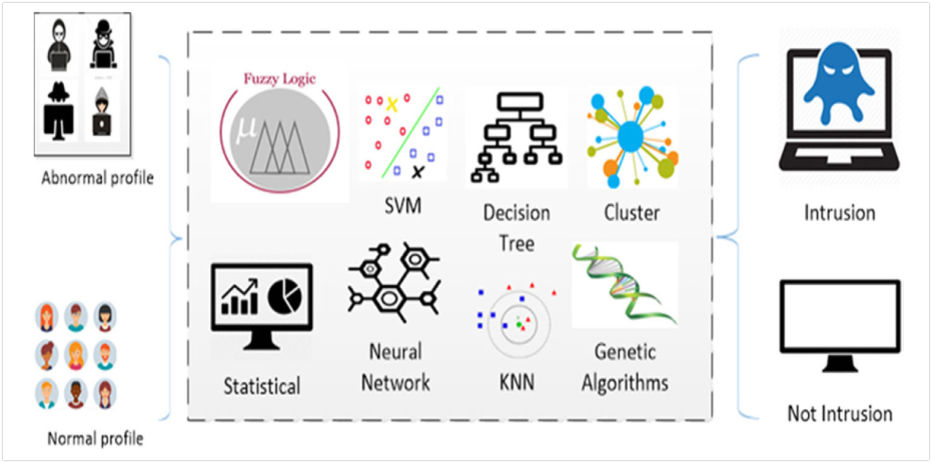
\includegraphics[scale=0.5]{ML_Algorithm.png}
        \caption{Machine Learning Algorithms}
        \label{fig:ML_Algorithm}
    \end{figure}

\end{frame}

\begin{frame}{Previous work}
    \begin{itemize}
        \item Mouhammed Alkasassbeh explained how they used Data mining techniques to detect Distributed Denial of Service (DDoS) Attacks. They identified UDP Flood, Smurf, SIDDoS, HTTPFlood
        \item Iman Sharafaldin et al.\citep{sharalfaldin2018} in their work, used CICFlowMeter to generate and extracted 80 traffic features from their dataset. They employed different classifiers including KNN, RF, ID3, Adaboost, MLP, Naïve-Bayes, and QDA. The performance report of their work showed varying results for Precision (Pr), Recall (Rc), F-Measure (F1), as well as execution time (in secs), which is given below.
    \end{itemize}
\end{frame}
\begin{frame}{Previous work}
     \begin{table}[bt]
    \begin{tabular}{|l|c|c|c|c|} \hline
    \textbf{Algorithm} & \textbf{Pr}
    & \textbf{Rc} & \textbf{F1} & \textbf{Execution(Sec.)} \\ \hline
    \uncover<2->{KNN} & \uncover<2->{0.96} & \uncover<2->{0.96} & \uncover<2->{0.96} & \uncover<2->{1908.23}\\
    \uncover<3->{RF} & \uncover<3->{0.98} & \uncover<3->{0.97} & \uncover<3->{0.97} & \uncover<3->{74.39}\\
    \uncover<4->{ID3} & \uncover<4->{0.98} & \uncover<4->{0.98} & \uncover<4->{0.98} & \uncover<4->{235.02}\\
    \uncover<5->{Adaboost} & \uncover<5->{0.77} & \uncover<5->{0.84} & \uncover<5->{0.77} & \uncover<5->{1126.24}\\
    \uncover<6->{MLP} & \uncover<6->{0.77} & \uncover<6->{0.83} & \uncover<6->{0.76} & \uncover<6->{575.73}\\
    \uncover<7->{Naive-Bayes} & \uncover<7->{0.88} & \uncover<7->{0.04} & \uncover<7->{0.04} & \uncover<7->{14.77}\\
    \uncover<8->{QDA} & \uncover<8->{0.97} & \uncover<8->{0.88} & \uncover<8->{0.92} & \uncover<8->{18.79}\\
    \hline
    \end{tabular}
    \end{table}

\end{frame}
\begin{frame}{Previous work}
    \begin{itemize}
        \item Leila et al carried out an extensive work on Intrusion Detection System using Convolutional Neural Network. A deep learning method that enables NIDS to detect the class of normal and abnormal data. 
        \item This approach employed Deep Leaning where there are hidden layers that perform a set of computation on the input data using some weights, bias and activation function.
        \item Ansam Khraisat et al., carried out a survey of IDS and outlined the challenges of each technique employed.\citep{Khraisat2019}

    \end{itemize}
\end{frame}

\begin{frame}{Research Focus}
    \begin{itemize}
        \item This research is aimed at using machine learning algorithms to identify and classify network attacks based on extracted features from network traffic. The goal is to develop a model that would classify raw network traffic data into various attack categories using similar approach and tune the data to achieve a more accurate result.
        \item Here, our focus is using a traffic generator CF20 from Spirent. We hope achieve better performance as this data is generated live and not simulated.
    \end{itemize}
\end{frame}

\begin{frame}{References}
    \bibliographystyle{plain}
\bibliography{references}
\end{frame}

\end{document}